\newcommand{\spywareTagResultsAucTable}{
    \begin{table}[H]
        \centering
        \begin{tabular}{|p{2,8cm}||P{2,2cm} P{2,2cm} P{2,2cm} P{2,2cm}|}
            \hline
            Spyware Tag & ALOHA\newline (M/B only) & ALOHA & Joint\newline Embedding & Proposed\newline Model \\
            \hline
            AUC-ROC & - & 0.959$\pm$0.005 & \textBF{0.971$\pm$0.001} & 0.968$\pm$0.001 \\
            \hline
        \end{tabular}
        \caption[Spyware Tag prediction task AUC-ROC results]{AUC-ROC (Area Under Curve) of the different models for the \textbf{Spyware Tag} prediction task. Results were aggregated over \textBF{3} training runs with different weight initializations and minibatch orderings. Best results are shown in \textbf{bold}.} \label{tab:spywareTag_auc}
    \end{table}
}

\newcommand{\spywareTagResultsAtFprTable}{
    \begin{center}
        \begin{longtable}[c]{|P{3,2cm}||P{1,8cm} P{1,8cm} P{1,8cm} P{1,8cm} P{1,8cm}|}
            \hline
            Spyware Tag & \multicolumn{5}{c|}{{FPR}} \\
            & $10^{-5}$ & $10^{-4}$ & $10^{-3}$ & $10^{-2}$ & $10^{-1}$ \\
            \hline
            \endfirsthead

            \caption*{\raggedright ...continued from previous page} \\
            \hline
            Spyware Tag & \multicolumn{5}{c|}{\textbf{FPR}} \\
            & $10^{-5}$ & $10^{-4}$ & $10^{-3}$ & $10^{-2}$ & $10^{-1}$ \\
            \hline
            \endhead

            \caption*{\raggedleft ...continued on next page} \\
            \endfoot

            \caption[Spyware Tag prediction task results]{Mean and standard deviation results (TPR, Accuracy, Recall, Precision and F1-Score) of the different models for the \textbf{Spyware Tag} prediction task at different \textbf{FPR}s (\textit{False Positive Rates}). Results were aggregated over \textBF{3} training runs with different weight initializations and minibatch orderings. Best results are shown in \textbf{bold}. Under \textbf{TPR} results are also presented the percentage reduction in mean detection error and in ROC curve standard deviation introduced by the \textit{Proposed Model} with respect to both \textit{ALOHA} model and \textit{Joint Embedding}.} \label{tab:spywareTag_results_at_fpr} \\
            \endlastfoot

            \multicolumn{6}{|c|}{\textbf{TPR}} \\
            \hline
            ALOHA (M/B only) & - & - & - & - & - \\
            ALOHA & \textBF{0.088$\pm$0.052} & 0.196$\pm$0.128 & 0.239$\pm$0.165 & 0.582$\pm$0.031 & 0.902$\pm$0.024 \\
            Joint Embedding & 0.013$\pm$0.004 & 0.214$\pm$0.101 & \textBF{0.398$\pm$0.151} & \textBF{0.688$\pm$0.033} & \textBF{0.922$\pm$0.009} \\
            Proposed Model & 0.044$\pm$0.026 & \textBF{0.246$\pm$0.159} & 0.363$\pm$0.060 & 0.660$\pm$0.003 & 0.887$\pm$0.016 \\
            \hline
            Error Reduction wrt\newline ALOHA (M/B only) & - & - & - & - & - \\
            Error Reduction wrt\newline ALOHA & -4.8\% & 6.2\% & 16.3\% & 18.7\% & -15.3\% \\
            Error Reduction wrt\newline Joint Embedding & 3.1\% & 4.1\% & -5.8\% & -9.0\% & -44.9\% \\
            \hline
            Std Reduction wrt\newline ALOHA (M/B only) & - & - & - & - & - \\
            Std Reduction wrt\newline ALOHA & 50.0\% & -24.2\% & 63.6\% & 90.3\% & 33.3\% \\
            Std Reduction wrt\newline Joint Embedding & -550.0\% & -57.4\% & 60.3\% & 90.9\% & -77.8\% \\
            \hline
            \multicolumn{6}{|c|}{\textbf{Accuracy}} \\
            \hline
            ALOHA (M/B only) & - & - & - & - & - \\
            ALOHA & \textBF{0.903$\pm$0.006} & 0.914$\pm$0.014 & 0.918$\pm$0.017 & 0.946$\pm$0.003 & 0.900$\pm$0.003 \\
            Joint Embedding & 0.894$\pm$0.000 & 0.916$\pm$0.011 & \textBF{0.935$\pm$0.016} & \textBF{0.958$\pm$0.004} & \textBF{0.902$\pm$0.001} \\
            Proposed Model & 0.898$\pm$0.003 & \textBF{0.919$\pm$0.017} & 0.931$\pm$0.006 & 0.955$\pm$0.000 & 0.899$\pm$0.002 \\
            \hline
            \multicolumn{6}{|c|}{\textbf{Recall}} \\
            \hline
            ALOHA (M/B only) & - & - & - & - & - \\
            ALOHA & \textBF{0.088$\pm$0.052} & 0.196$\pm$0.128 & 0.239$\pm$0.166 & 0.582$\pm$0.031 & 0.902$\pm$0.024 \\
            Joint Embedding & 0.012$\pm$0.004 & 0.214$\pm$0.101 & \textBF{0.398$\pm$0.151} & \textBF{0.688$\pm$0.033} & \textBF{0.922$\pm$0.009} \\
            Proposed Model & 0.044$\pm$0.026 & \textBF{0.246$\pm$0.159} & 0.363$\pm$0.060 & 0.660$\pm$0.003 & 0.887$\pm$0.016 \\
            \hline
            \multicolumn{6}{|c|}{\textbf{Precision}} \\
            \hline
            ALOHA (M/B only) & - & - & - & - & - \\
            ALOHA & \textBF{0.998$\pm$0.002} & 0.993$\pm$0.005 & 0.950$\pm$0.037 & 0.874$\pm$0.006 & 0.519$\pm$0.007 \\
            Joint Embedding & 0.997$\pm$0.003 & \textBF{0.994$\pm$0.004} & 0.975$\pm$0.012 & \textBF{0.892$\pm$0.004} & \textBF{0.524$\pm$0.002} \\
            Proposed Model & 0.996$\pm$0.004 & 0.990$\pm$0.011 & \textBF{0.977$\pm$0.004} & 0.888$\pm$0.000 & 0.515$\pm$0.004 \\
            \hline
            \multicolumn{6}{|c|}{\textbf{F1 Score}} \\
            \hline
            ALOHA (M/B only) & - & - & - & - & - \\
            ALOHA & \textBF{0.158$\pm$0.091} & 0.307$\pm$0.195 & 0.352$\pm$0.234 & 0.698$\pm$0.025 & 0.659$\pm$0.012 \\
            Joint Embedding & 0.025$\pm$0.008 & 0.340$\pm$0.146 & \textBF{0.548$\pm$0.167} & \textBF{0.777$\pm$0.022} & \textBF{0.669$\pm$0.004} \\
            Proposed Model & 0.082$\pm$0.048 & \textBF{0.366$\pm$0.223} & 0.526$\pm$0.065 & 0.757$\pm$0.002 & 0.651$\pm$0.008 \\
            \hline
        \end{longtable}
    \end{center}
}

\newcommand{\spywareTagResultsSummaryTable}{
    \begin{table}[H]
        \centering
        \begin{tabular}{|P{3,2cm}||P{1,8cm} P{1,8cm} P{1,8cm} P{1,8cm} P{1,8cm}|}
            \hline
            \multicolumn{6}{|c|}{Spyware Tag (at FPR $=1\%$)} \\
            \hline
            Model & TPR & Accuracy & Precision & Recall & F1 score \\
            \hline
            ALOHA (M/B only) & - & - & - & - & - \\
            ALOHA & 0.582$\pm$0.031 & 0.946$\pm$0.003 & 0.874$\pm$0.006 & 0.582$\pm$0.031 & 0.698$\pm$0.025 \\
            Joint Embedding & \textBF{0.688$\pm$0.033} & \textBF{0.958$\pm$0.004} & \textBF{0.892$\pm$0.004} & \textBF{0.688$\pm$0.033} & \textBF{0.777$\pm$0.022} \\
            Proposed Model & 0.660$\pm$0.003 & 0.955$\pm$0.000 & 0.888$\pm$0.000 & 0.660$\pm$0.003 & 0.757$\pm$0.002 \\
            \hline
        \end{tabular}
        \caption[Summary of Spyware Tag prediction task results]{Summary of the mean and standard deviation results of the different models for the \textbf{Spyware Tag} prediction task at \textbf{FPR} $=1\%$. Results were aggregated over \textBF{3} training runs with different weight initializations and minibatch orderings. Best results are shown in \textbf{bold}.} \label{tab:spywareTag_result_summary}
    \end{table}
}

\newcommand{\spywareTagRocAlohaMB}{
    \begin{figure}[H]
        \vspace*{-0.5cm}
        \centering
        \includegraphics[width=0.6\textwidth]{./results/spyware_tag_roc_alohaMB.png}
        \vspace*{-0.2cm}
        \caption[Spyware Tag prediction task ALOHA (M/B only) ROC curve]{ROC curve and AUC statistics of \textBF{ALOHA (M/B only)} model for the \textbf{Spyware Tag}. The line represents the \textit{mean} TPR at a given FPR, while the shaded region represents the \textit{standard deviation}. Statistics were computed over \textBF{3} training runs, each with random parameter initialization.}
        \label{fig:spywareTagRocAlohaMB}
    \end{figure}
}

\newcommand{\spywareTagRocAloha}{
    \begin{figure}[H]
        \vspace*{-0.5cm}
        \centering
        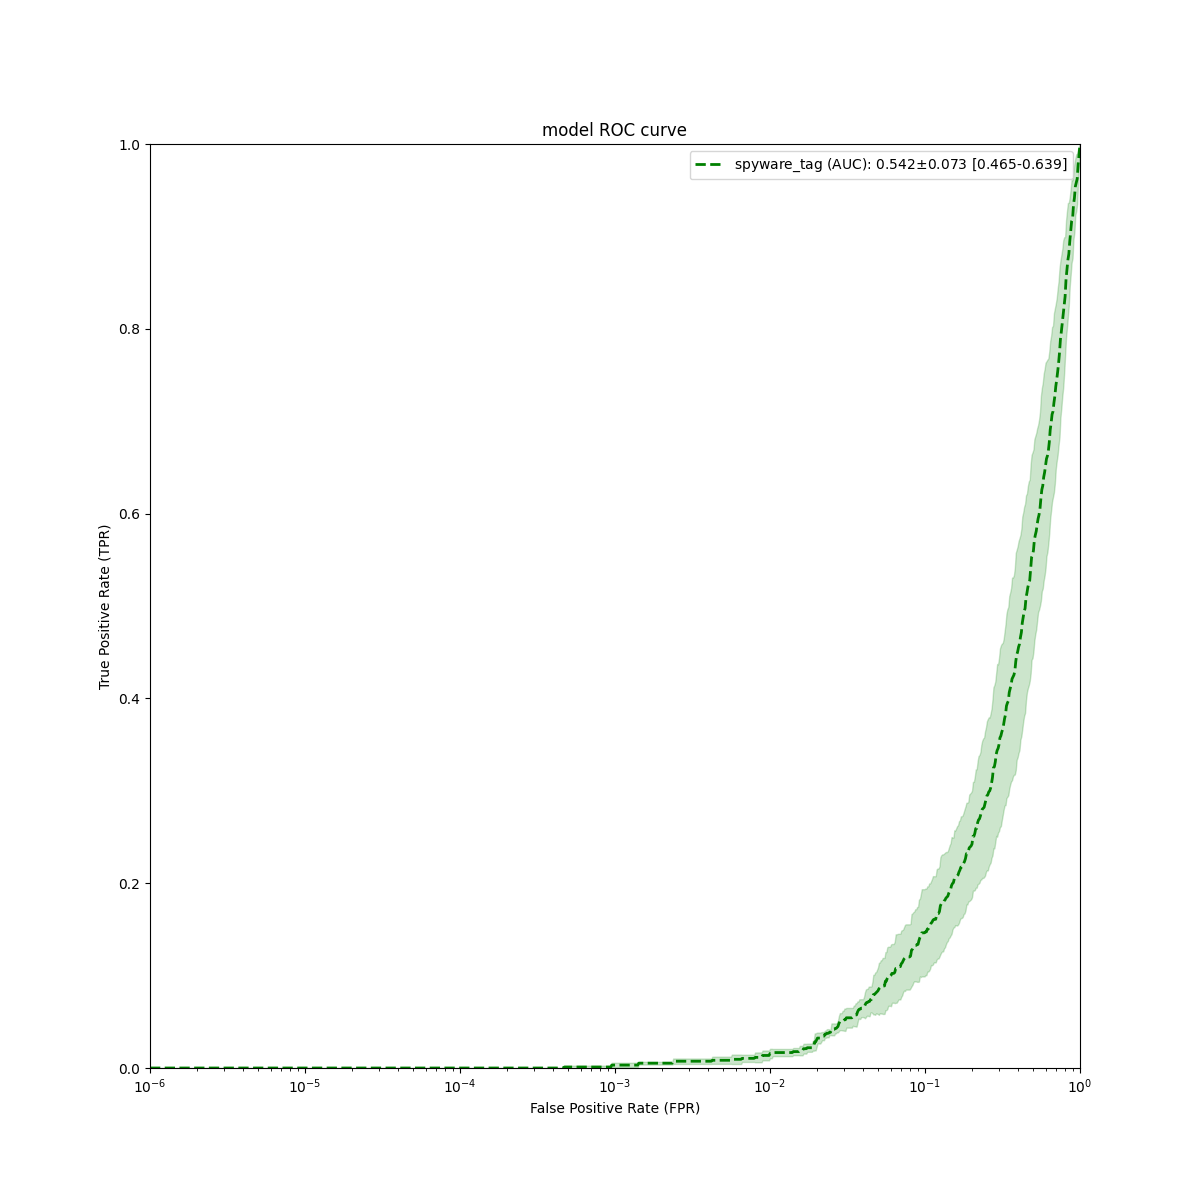
\includegraphics[width=0.6\textwidth]{./results/spyware_tag_roc_aloha.png}
        \vspace*{-0.2cm}
        \caption[Spyware Tag prediction task ALOHA ROC curve]{ROC curve and AUC statistics of \textBF{ALOHA} model for the \textbf{Spyware Tag}. The line represents the \textit{mean} TPR at a given FPR, while the shaded region represents the \textit{standard deviation}. Statistics were computed over \textBF{3} training runs, each with random parameter initialization.}
        \label{fig:spywareTagRocAloha}
    \end{figure}
}

\newcommand{\spywareTagRocJointEmbedding}{
    \begin{figure}[H]
        \vspace*{-0.5cm}
        \centering
        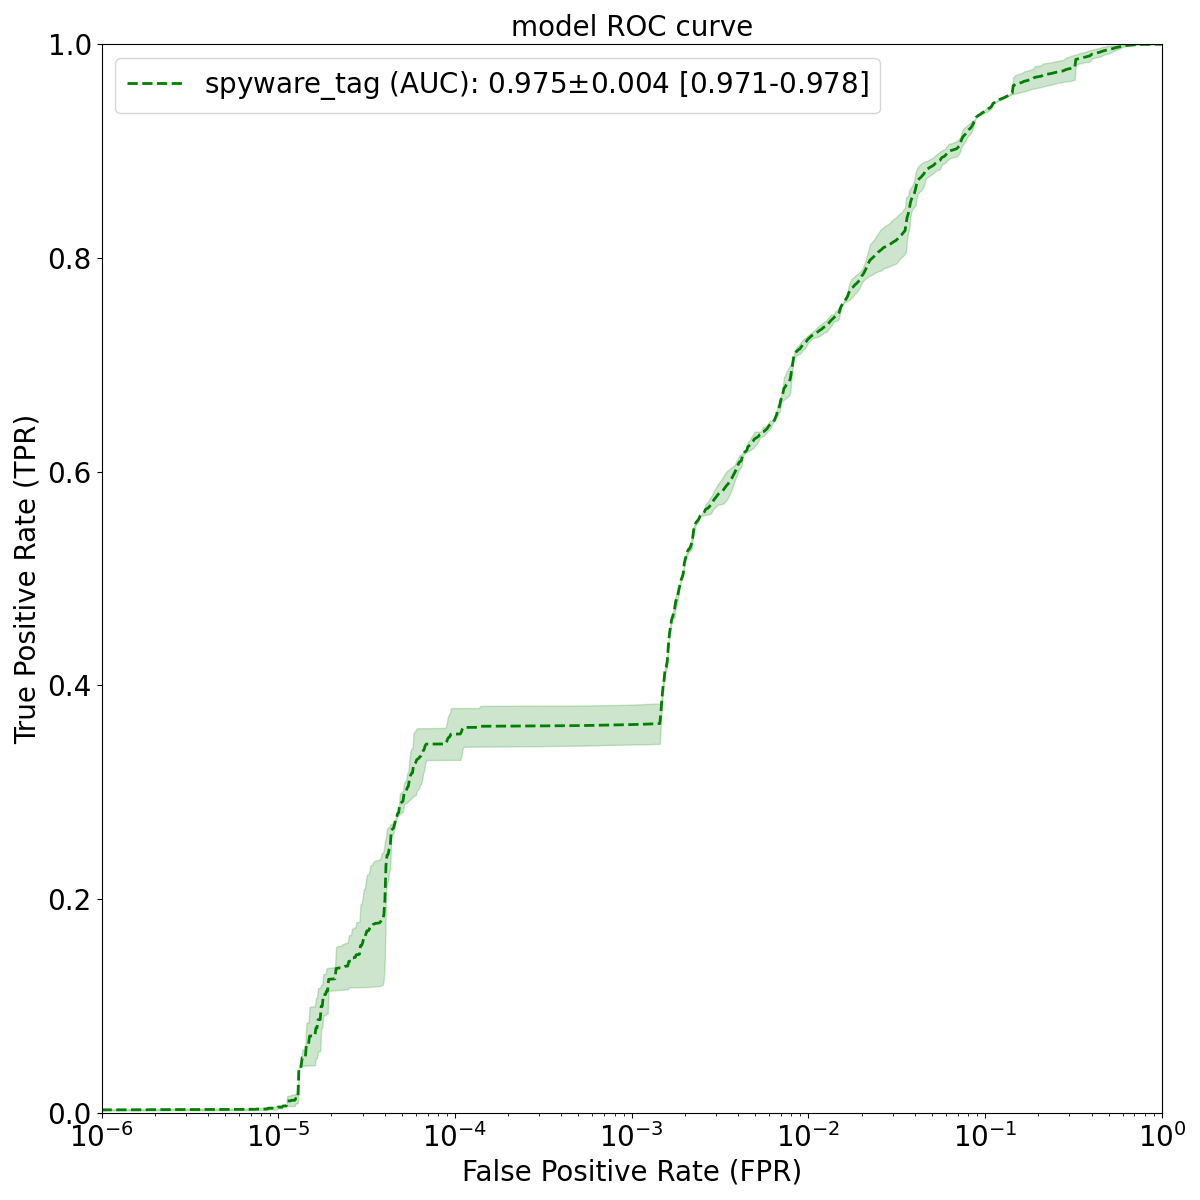
\includegraphics[width=0.6\textwidth]{./results/spyware_tag_roc_jointEmbedding.png}
        \vspace*{-0.2cm}
        \caption[Spyware Tag prediction task Joint Embedding ROC curve]{ROC curve and AUC statistics of \textBF{Joint Embedding} model for the \textbf{Spyware Tag}. The line represents the \textit{mean} TPR at a given FPR, while the shaded region represents the \textit{standard deviation}. Statistics were computed over \textBF{3} training runs, each with random parameter initialization.}
        \label{fig:spywareTagRocJointEmbedding}
    \end{figure}
}

\newcommand{\spywareTagRocProposedMethod}{
    \begin{figure}[H]
        \vspace*{-0.5cm}
        \centering
        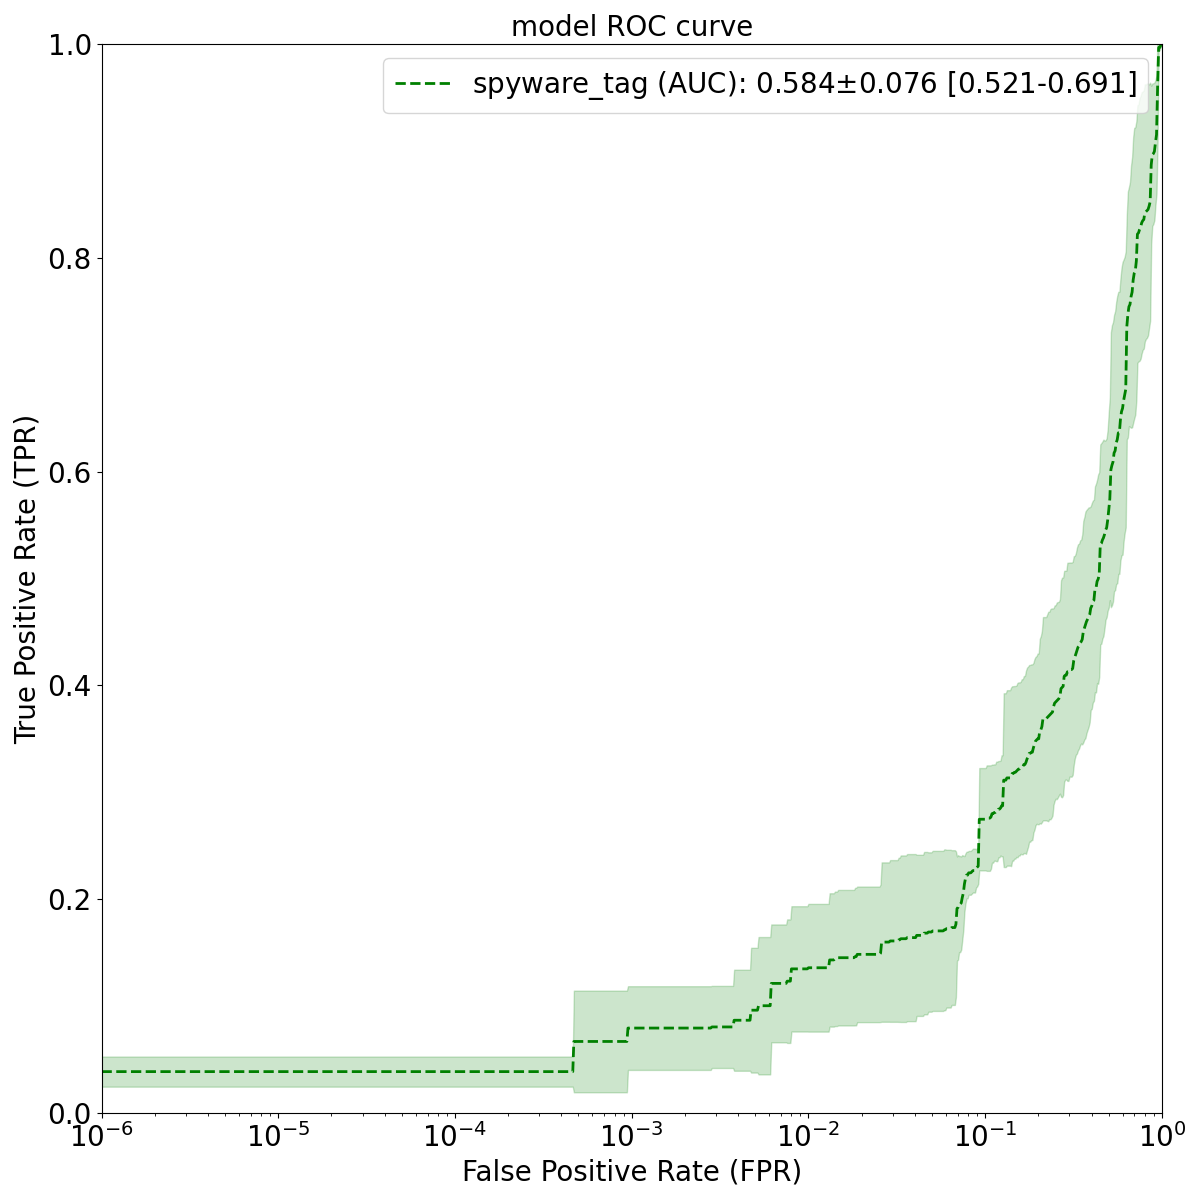
\includegraphics[width=0.6\textwidth]{./results/spyware_tag_roc_proposedModel.png}
        \vspace*{-0.2cm}
        \caption[Spyware Tag prediction task Proposed Model ROC curve]{ROC curve and AUC statistics of \textBF{Proposed Model} for the \textbf{Spyware Tag}. The line represents the \textit{mean} TPR at a given FPR, while the shaded region represents the \textit{standard deviation}. Statistics were computed over \textBF{3} training runs, each with random parameter initialization.}
        \label{fig:spywareTagRocProposedModel}
    \end{figure}
}
